%%%%%%%%%%%%%%%%%%%%%%% file template.tex %%%%%%%%%%%%%%%%%%%%%%%%%
%
% This is a general template file for the LaTeX package SVJour3
% for Springer journals.          Springer Heidelberg 2010/09/16
%
% Copy it to a new file with a new name and use it as the basis
% for your article. Delete % signs as needed.
%
% This template includes a few options for different layouts and
% content for various journals. Please consult a previous issue of
% your journal as needed.
%
%%%%%%%%%%%%%%%%%%%%%%%%%%%%%%%%%%%%%%%%%%%%%%%%%%%%%%%%%%%%%%%%%%%
%
% First comes an example EPS file -- just ignore it and
% proceed on the \documentclass line
% your LaTeX will extract the file if required
\begin{filecontents*}{example.eps}
%!PS-Adobe-3.0 EPSF-3.0
%%BoundingBox: 19 19 221 221
%%CreationDate: Mon Sep 29 1997
%%Creator: programmed by hand (JK)
%%EndComments
gsave
newpath
  20 20 moveto
  20 220 lineto
  220 220 lineto
  220 20 lineto
closepath
2 setlinewidth
gsave
  .4 setgray fill
grestore
stroke
grestore
\end{filecontents*}
%
\RequirePackage{fix-cm}
%
%\documentclass{svjour3}                     % onecolumn (standard format)
%\documentclass[smallcondensed]{svjour3}     % onecolumn (ditto)
\documentclass[smallextended]{svjour3}       % onecolumn (second format)
%\documentclass[twocolumn]{svjour3}          % twocolumn
%
\smartqed  % flush right qed marks, e.g. at end of proof
%
\usepackage{graphicx}
%
% \usepackage{mathptmx}      % use Times fonts if available on your TeX system
%
% insert here the call for the packages your document requires
%\usepackage{latexsym}
% etc.
%
% please place your own definitions here and don't use \def but
% \newcommand{}{}
%
% Insert the name of "your journal" with
% \journalname{myjournal}
%
\begin{document}

\title{Hardware Reconfiguration Scheme Based on the Digital TV Signal%\thanks{Grants or other notes
%about the article that should go on the front page should be
%placed here. General acknowledgments should be placed at the end of the article.}
}
%\subtitle{Do you have a subtitle?\\ If so, write it here}

%\titlerunning{Short form of title}        % if too long for running head

\author{Rodrigo Oliveira \and
        Lucas Cordeiro \and
				Eddie de Lima Filho and \and %etc.
				Vicente de Lucena Jr. \and
}

%\authorrunning{Short form of author list} % if too long for running head

\institute{Rodrigo Oliveira \at
              Computer Institute, Federal University of Amazonas, Manaus, Brazil \\
              Tel.: +55-11-45318412\\
              Fax: +55-11-45318412\\
              \email{rodrigo@dcc.ufam.edu.br}           %  \\
%             \emph{Present address:} of F. Author  %  if needed
           \and
           S. Author \at
              second address
}

\date{Received: 20 August 2015 / Accepted: date}
% The correct dates will be entered by the editor


\maketitle

\begin{abstract}
This work presents a new hardware reconfiguration approach, named hardware reconfiguration through digital television (HARD), which is capable of updating hardware modules, based on the digital TV (DTV) signal content. Such a scheme allows several synthesized hardware cores (bit-streams) to be signaled and simply broadcast, through an open DTV signal. Service information content, specifically designed for identifying and describing characteristics of the multiplexed hardware bit-streams, is added to the transmitted signal. The receiver framework, in turn, checks whether those characteristics correspond to its embedded reconfigurable devices and, if a match is found, it reassembles the related bit-streams and reconfigures the respective devices. HARD can be used in several designs, regarding intelligent reconfigurable devices, and has the potential to minimize device costs and provide a better hardware reuse.
\keywords{Digital TV \and TV receivers \and Programmable circuits \and Programmable logic arrays.}
% \PACS{PACS code1 \and PACS code2 \and more}
% \subclass{MSC code1 \and MSC code2 \and more}
\end{abstract}

\section{Introduction}
\label{intro}
%Your text comes here. Separate text sections with
Embedded systems, as well as digital TV (DTV) receivers, are designed with no concern for technology advancements, regarding computational tasks performed by hardware, over time. Such systems typically have several functions performed with silicon hardware (application specific integrated circuit - ASIC), because they demand high computational complexity. One example of that is video decoding ({\em e.g.}, advanced video coding - AVC or AVC/H.264~\cite{ref1}), which is a demanding task normally performed by an ASIC silicon device.

Typically, when a new DTV network is deployed, ASIC devices are then used for developing new receivers, which provide all necessary decoding/processing techniques. However, if the associated standard is revised and other algorithms and/or protocols are adopted, the current infrastructure must be replaced. Such a problem is commonly known as hardware legacy and is closely related to the use of ASICs.

Recently, the international telecommunications union (ITU) introduced the high efficiency video coding (HEVC), also known as HEVC/H.265~\cite{ref2,ref3}, as the next-generation video compression standard. Compared with its predecessor (MPEG-4 AVC/H.264), it presents about twice the compression efficiency, without deteriorating the quality level of the encoded signal~\cite{ref4}.

Given what was presented, one may notice that AVC/H.264-based systems are unable to incorporate the benefits of HEVC/H.265 immediately, due to hardware legacy. However, such flexibility could be achieved if the DTV receiver architecture was capable of performing demanding tasks through reconfigurable devices ({\em e.g.}, field programmable gate array - FPGA), instead of ASICs.

Currently, the semiconductor industry and open core communities have boosted the use of FPGA. The latter even provide hardware-description source codes ({\em e.g.}, VHSIC hardware description language - VHDL~\cite{ref5} and Verilog~\cite{ref6}), for a number of applications ({\em e.g.}, crypto cores, DSP cores and encoder/decoder cores), which are available for download and immediate use in project solutions~\cite{ref7}.

Furthermore, current FPGA technologies are already a good option, when compared to ASICs, due to price equalization between them, which is provided by the amortization of non-recurring engineering (NRE) costs among customers, for each integrated circuit (IC) family~\cite{ref8,ref9}. This reinforces the development of hardware architectures and critical tasks using reconfigurable devices, in embedded systems. 

The growth in the adoption of FPGA solutions can already be seen in various segments of the consumer electronics industry~\cite{ref10}, especially DTV, where such devices are used for implementing specific functions in corresponding receivers ({\em e.g.}, timing control and output interfaces)~\cite{ref11}.

Although FPGA solutions are very interesting and present many advantages, one may argue that, in horizontal markets, competition is very intense and set-top boxes (STB) present low profit margins, which would prevent manufacturers from including extra hardware in their products. In addition, mobile receivers also present cost and power consumption restrictions. Nonetheless, in vertical markets, cable and satellite operators must provide receivers to all subscribers, in order to offer services. Besides, if the underlying technology advances, new receivers are needed, which is very expensive. As a consequence, the proposed approach could bring a lot of benefits to pay TV operators, since it may be cheaper to update receivers instead of replacing them.

The observations presented in the last paragraphs are the inspiration for the present work, which proposes a new approach for hardware update, with the DTV signal as transport infrastructure, named hardware reconfiguration through digital television (HARD). In the context of a DTV system, the reconfiguration bit-stream can be regarded as regular data broadcast, along with the high definition television (HDTV) content of a television program, as shown in Fig.~\ref{figure:fig1}. A DTV system is composed of several subsystems, which include data preparation for transmission and complete signal reception, with subsequent content filtering. In the transport stream (TS) step, audio, video, and data, which include the FPGA bit-stream, are interleaved, engendering a multiplexed DTV stream flow~\cite{ref12}. Finally, in the transmission step, the resulting signal is then modulated and sent through a DTV channel. At the receiving side (see Fig.~\ref{figure:fig1}), each device in range detects and decodes the transmitted content. The result of this process is the complete extraction of the FPGA-core data stream, which is then reassembled in a persistent storage module. After this step, the FPGA module is reconfigured.

%
\begin{figure}[ht]
\centering
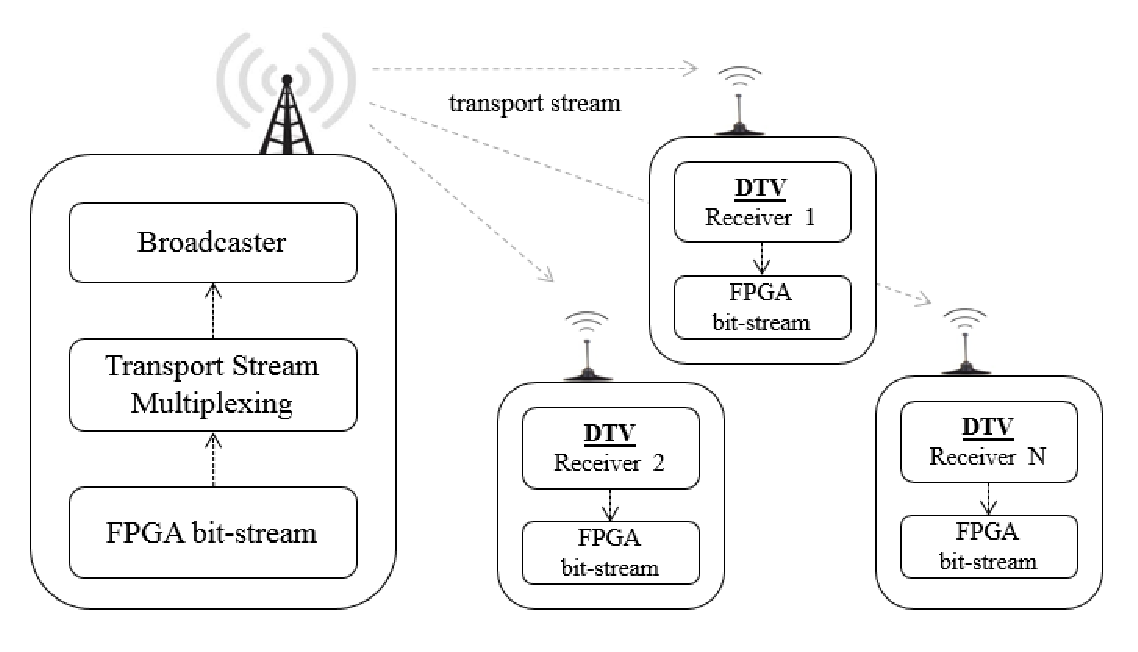
\includegraphics[width=3.4in]{images/Fig1.eps}
\caption{The FPGA bit-stream broadcast, in a DTV environment.}
\label{figure:fig1}
\end{figure}
%

This work deals with generic hardware update for DTV environments, where receivers do not need to leave the user premises. Indeed, designing reconfigurable hardware architectures can be an efficient way to improve the receiver lifespan, or even to create low cost receivers  and embedded systems (depending on the target market).

The presented scheme extends the use of DTV channels, introducing a way of transmitting synthesized hardware data. It can be employed in a wide range of future designs, regarding intelligent hardware architectures, and has the potential to boost the use of hardware reconfiguration in embedded solutions ({\it e.g.}, DTV receivers), besides providing the opportunity to deeply exploit this scheme, in order to develop reconfigurable architectures.

Hardware reconfiguration has already been used in a vast range of projects, but the solution presented here is an innovative way to perform this process. It is expected that the subject of this work, along with its related schema, can stimulate the scientific community to develop a wide range of environments, which rely on the hardware update technology.

The remaining of this work is organized as follows. Section \ref{related-work} provides a summary regarding the related literature. Section \ref{hardware-data} contains a brief explanation of DTV and data broadcasting. Next, section \ref{dtv-receiver} tackles reference receivers and basic concepts related to FPGA configuration schemes. Then, section \ref{hardware-reconfig} presents the complete hardware update approach, by detailing each step involved in this process. Finally, conclusions and future work are presented in section \ref{conclu}.


%==============================================================
\section{Related Work}
\label{related-work}
%==============================================================

Recent studies, on similar topics, present some related work based on intelligent hardware architectures, with hardware reconfiguration, as the core technology, for building more compact and efficient systems.
Indeed, architectures with hardware resource management present a new trend in embedded systems. In these approaches, pre-synthesized hardware unit functions are able to execute run-time reconfiguration of FPGA cores, according to the user's interaction, such as described by Lin {\em et al}~\cite{ref13}.  
This work presents a hybrid architecture that uses a CPU and a reconfigurable device (FPGA) for performing tasks. Such a system is controlled by a resource manager that uses a decision algorithm to choose among pre-synthesized hardware cores or software modules, which are kept in a resource queue. When the mentioned resource manager indicates the use of a hardware module, the FPGA is reconfigured; otherwise, a software module is run by the CPU and performs the desired task.

Intelligent embedded systems can make use of partial dynamic hardware, for run-time reconfiguration. Such a feature, which is similar to a microprocessor multi-task system, allows a multiplex of distinct hardware modules to run at the same time. Thus, functional pre-synthesized hardware blocks, {\em i.e.}, logical blocks, can be reconfigured or not, according to system needs~\cite{ref14}. The associated system architecture is coordinated by a microcontroller device, which is in charge of reconfiguring pre-synthesized hardware blocks in the FPGA device. In addition, a list of pre-synthesized hardware blocks are kept in flash memory. This way, the use of partial dynamic reconfiguration causes a considerable reduction in power consumption, besides a significant decrease in device costs.

The reconfigurable streaming architecture, presented by Hillenbrand {\em et al}~\cite{ref15}, allows the inclusion of signal-processing pre-synthesized cores, into hardware description language (HDL) sources, to be run-time reconfigurable. Such a feature is very important, considering that state-of-the-art FPGA devices require large amounts of time and memory for their compilation processes. In those cases, the pre-synthesized cores minimize the synthesis process and allow the design of adaptive reconfigurable system architectures. 

A complete multi-core reconfigurable platform, combining processors with some reconfigurable logic, can provide a rich and flexible environment for application programmers, as proposed by Serres {\em et al}~\cite{ref16}. In this architecture, each processor core has a coupled reconfigurable coprocessor unit, which allows the extension of the processor instruction set for running applications.

A streaming-based partially reconfigurable architecture and programming model may be used to simplify the development of streaming applications. Thus, programmers could describe streaming applications based on a unified software/hardware multithread model. The efficiency presented by such a reconfigurable architecture demonstrate that the power efficiency is much better than that of state-of-the-art GPUs~\cite{refX1}.

The shown related works are based on pre-synthesized cores, which need to be present on their embedded file systems. Those cores are used according to system demands, or even due to user interaction. However, HARD is based on broadcast networks, through which pre-synthesized cores, for updating several devices, can be sent. Therefore, several core modules, from different manufacturers, can be delivered at the same time, for a large amount of receivers.

Hardware reconfiguration techniques can be used in a wide variety of applications, in such a way that a specific feature can be updated or even integrated into a given platform, as seen above. Regarding video decoding, a similar result may be achieved with the reconfigurable video coding (RVC) framework \cite{ref34,ref40}, which provides coding specifications based on library components, instead of monolithic solutions. In summary, a coding problem can be tackled by selecting components of a standard coding-algorithm library, so that a specific solution may be assembled. Such an approach has the potential to even provide more flexibility on the choice of the coding-tool subset (profile), which already exists in current standards, given that it already presents some drawbacks, due to the lack of optimal solutions for many specific cases. The decoder model is provided via a specific language called Cal, which employs notions of actor programming and dataflow \cite{ref34,ref37}. There are also synthesis approaches \cite{ref37,ref35,ref36,ref39,ref41}, which are able to covert high-level descriptions to C or HDL code. Additionally, reconfigurable/multi-standard platforms \cite{ref38} can be developed, with the potential to reduce the hardware legacy problem.

Based on what was presented, the relation between HARD and RVC can be analyzed from two different aspects. First, with an initial library of video coding-algorithms, an arbitrary combination of standardized basic coding algorithms can be obtained \cite{ref34}, which would provide optimal configurations for specific scenarios and indeed achieve the same goal of the proposed solution. The main difference here is that while RVC relies on a reconfiguration procedure regarding existing tools (which is a flexible approach), HARD would need a new hardware description to be transmitted; however, the latter has the potential to use less system resources ({\it e.g.}, memory and gates), when compared to RVC. In addition, receivers must be updated before receiving content coded with new algorithms, while RVC bit-streams carry all necessary information for decoding. Second, even that initial library will need to be updated, with new coding tools for enhanced performance or different coding paradigms. Thus, one may notice that the RVC framework and HARD become complementary solutions, given that new modules could be generated and then transmitted and updated through the framework presented here. It is worth noticing that the mentioned synthesis tools \cite{ref35} can be used for generating a target decoder, based on the Cal description. Then, the resulting HDL module could be transmitted and used to update all available decoders, using HARD, in a similar way as in direct download applications \cite{ref34}.

%==============================================================
\section{Hardware-Data Broadcast Through The Digital TV Signal}
\label{hardware-data}
%==============================================================

The DTV TS consists of packets with audio, video, and data, which are $188$ bytes in length. The packet is the basic TS data unit and is composed of a sync-byte field, whose value is 0x47, followed by three $1$-bit fields (transport error indicator, payload unit start indicator, and transport priority) and an identification ($13$-bit), known as packet identifier (PID)~\cite{ref17}, among others. The PID provides a means of differentiating the payload content of each transport unit (packet), in a TS; if a PID is allocated and reported to a receiver (through a table), this means that a given packet carries video, audio, or other data, according to what was informed. Thus, the proprietary broadcast content is identified by its respective PID values.

Fig.~\ref{figure:fig2} shows a representation of a transport stream with different packets, which consist of video, audio, program association table (PAT), and hardware payload (PID 0x77). This transport stream slice shows that packets with the same PID, that is, carrying parts of the same information, are spaced over time. The receiver demultiplexer then needs to filter a transport stream, using the corresponding PIDs, for accessing its payload content.

%
\begin{figure}[ht]
\centering
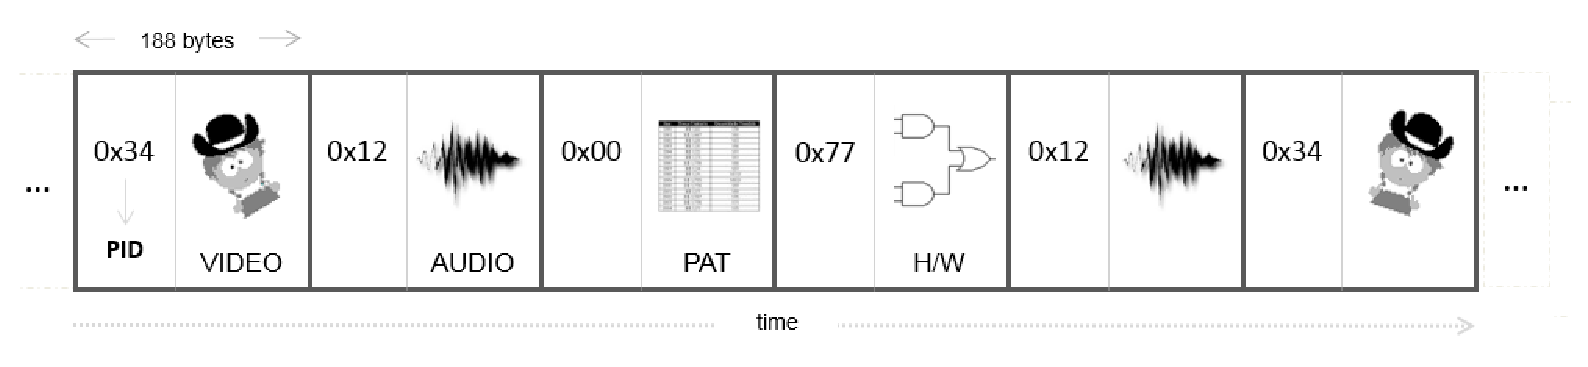
\includegraphics[width=3.4in]{images/Fig2.eps}
\caption{Transport stream packet structure used to carry different data types, which include hardware reconfiguration data.}
\label{figure:fig2}
\end{figure}
%

The DTV system is able to broadcast binary applications~\cite{ref17}, which are interleaved with other HDTV contents (audio, video, and data). In order to inform that an application is being broadcast, the DTV standard uses the application information table (AIT)~\cite{ref18}. The AIT information is used, by the receiver resident system, for downloading all content related to the associated application.

The DTV telecommunication network allows the broadcast of several data types. Here, it is important to consider two main characteristics: the data format and the required synchronization, which are necessary for broadcasting some data types. The format may be classified into three categories, as follows: delimited data, un-delimited data, and datagrams following some protocol control. The delimited data can be divided into units of a defined size ({\em e.g.}, files and objects); however, the un-delimited data are considered continuous bit-streams. Finally, datagrams correspond to data packets related to a communication protocol ({\em e.g.}, IPv4 and IPv6).

Regarding synchronization, transmitted data are divided into synchronous, synchronized, and asynchronous~\cite{ref19}. The synchronous data have synchronization requirements with other data in the same stream, which is known as intra-media synchronization. Synchronized data are those that must be presented at predetermined time instances and in synchronism with elements of other media ({\em e.g.}, closed caption), which is called inter-media synchronization. Finally, the asynchronous data, in turn, have no temporal synchronization requirements. 

The data format characteristics and the required data synchronization are important to consider, when choosing the best way for data broadcasting.

%==============================================================
\subsection{Data Broadcasting Mechanisms}
\label{data-broadcasting}
%==============================================================

An important feature of DTV standards is the data broadcasting capability. The broadcast data are normally used to describe and identify the HDTV broadcast content. For instance, the European DTV standard, known as digital video broadcasting (DVB), offers four data transport mechanisms: data piping, data streaming, multiprotocol encapsulation (MPE), and Carousels~\cite{ref20,ref21}. Data piping is the simplest mechanism, which consists of inserting raw data directly into the TS packet payload area. Data streaming is more complex, when compared to the data piping method. The data streaming approach can arrange data using private sections or packetized elementary stream (PES) packets. Private sections are split into $4084$ bytes of payload, plus $8$ bytes of header and $4$ bytes of cyclic redundancy check (CRC), which amounts to $4096$ bytes. Some advantages regarding private sections are the contiguity control, given by the section number field, and the error detection control, which is obtained via redundant information ({\em e.g.}, CRC\_32)~\cite{ref22}. Reimers describes the data streaming method by PES packets~\cite{ref23}. MPE uses the logical link control sub-network access protocol (LLC/SNAP) encapsulation, which allows the use of any network protocol. Particularly, MPE allows the use of unicast ({\em i.e.}, datagram sent to a single receiver) and multicast ({\em i.e.}, datagram sent to receiver sets). Carousels are techniques used to repeatedly deliver data in a continuous cycle ~\cite{ref24,ref25}, as defined by the digital storage media command and control (DSM-CC) standard~\cite{ref26}, which is adopted by both digital audio video council (DAVIC) and DVB. DSM-CC specifies two types of carousels: data and object carousels. The latter extends the data carousel by specifying a file system directory structure ({\em e.g.}, media files, applications, image files, and directories). Section V-A addresses the presented broadcasting methods, by evaluating the core data characteristics and the most suitable method to implement hardware reconfiguration schemes.

%==============================================================
\section{DTV Receiver Architectures and FPGA Reconfiguration Schemes}
\label{dtv-receiver}
%==============================================================

DTV receivers ({\em e.g.}, Set-top Boxes) are used to demodulate and decode the HDTV broadcast signal, in such a way that the transmitted TS, carrying audio, video, and data packets (see section \ref{hardware-data}) is recovered. Normally, DTV standards specify reference receiver architectures, in order to suggest design implementations to manufacturers~\cite{ref27}. In fact, commercially available receivers normally present similar composition and provide a set of device drivers with exemplary applications. These data are taken as a reference to access and manipulate hardware devices. 

Fig.~\ref{figure:fig3} shows the basic components present in receiver architectures. The air interface ({\em e.g.}, front-end, also called tuner) device is responsible for demodulating any available DTV signal, in the receiver range. It recovers the TS stream flow output by the multiplexer device, which was sent at the transmitter end. The DEMUX component uses the front-end (air interface) output (a transport stream flow), splits packets related to a given PID identifier (see section \ref{hardware-data}), and outputs them in continuous separate flows. Later on, those flows are forwarded to their respective decoders ({\it e.g.}, H.$264$ video decoder), which in turn decode the content ({\em e.g.}, audio or video packets), in a continuous decoding process. Finally, the information output by the video decoder is passed to its respective digital video encoder (DENC) module, which converts digital baseband video data into analog signals ({\it e.g.}, Y/C and composite video broadcast signal), in order to provide video interface with other equipment ({\it e.g.}, television sets and personal video recorders). The other flows, present in the transport stream, are split by DEMUX, according to a given PID provided by the resident application ({\em e.g.}, filter software parser) control.

%
\begin{figure}[ht]
\centering
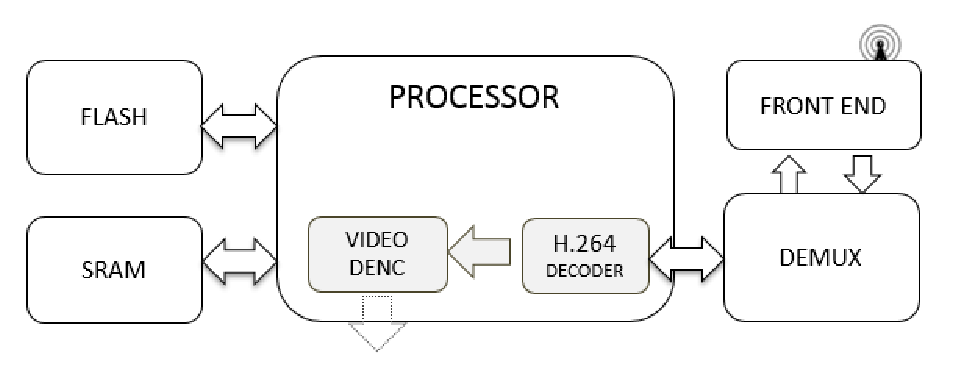
\includegraphics[width=3.4in]{images/Fig3.eps}
\caption{Receiver architecture composed of air interface (Front-end), demultiplexer, H.264 decoder, and memory.}
\label{figure:fig3}
\end{figure}
%

%==============================================================
\subsection{FPGA Standalone Reconfiguration Schemes}
\label{fpga-standalone}
%==============================================================

The standard process of hardware development begins with a design entry ({\em e.g.}, hardware schematics or HDL)~\cite{ref28}. Then, a HDL is used for developing hardware specifications to configure a FPGAs or a complex programmable logic device (CPLD). The most well-known HDLs are VHDL and Verilog. In the final step of the design flow, a bit-stream file ({\em e.g.}, raw binary file - RBF) is generated, which is then used to reconfigure the FPGA device. Typically, it is done by an electronic design automation (EDA) tool, which is also provided by the FPGA manufacturer~\cite{ref28}. Thus, it is possible to validate the final design behavior before delivering the bit-stream.

Although the FPGA reconfiguration is done by a tool, typically provided by the manufacturer, one may also develop a standalone reconfiguration scheme. In general, standalone schemes employ two modes ({\em e.g.}, master or slave modes) to reconfigure the FPGA, using a bit-stream (pre-synthesized binary code). In master mode, an FPGA is typically used to control the reconfiguration process; however, in slave mode, the FPGA configuration is controlled by an external device ({\em e.g.}, microcontroller, CPLD, or another FPGA). Additionally, the standard IEEE $1149.1$~\cite{ref29}, known as joint test action group (JTAG), is another mode commonly used by FPGA manufacturers. Normally, FPGA manufacturers provide a JTAG cable along with a programming tool, which is used to reconfigure their FPGA development boards. These cables are available to work with different communication interfaces, such as USB, parallel/serial port, or ethernet and are an attractive way to construct a host/target communication interface. This interface is commonly adopted by several embedded systems and has already been largely tested and validated. The JTAG has basically $4$ control signals: test data input (TDI), test data output (TDO), test mode select (TMS), and test clock (TCK), which are used to configure the device through a test access port (TAP) controller~\cite{ref29}. 

The literature also presents standalone open-source JTAG libraries~\cite{ref30,ref31} that enable a variety of JTAG-based manufacturer communication cables. Those libraries can use the serial vector format (SVF)~\cite{ref32}, in order to configure several FPGA models. The SVF file, which describes actions over JTAG interfaces, is a standard used for exchanging descriptions of high-level IEEE 1149.1 (JTAG) bus operations~\cite{ref32}. The standalone program can parse and play the SVF file, thus reconfiguring the FPGA.

SVF files can be obtained from other formats, through a converting tool or even an FPGA manufacturer tool. Indeed, most FPGA manufacturers commonly provide this file, which is used as a standard format to reconfigure devices.

In order to create a host/target physical connection, the reference DTV receiver was used as host device, and a commercial FPGA board as target device. The USB-manufacturer programmer cable, based on the JTAG program mode, is used to connect both sides, as seen in Fig.~\ref{figure:fig4}.

The standalone FPGA programmer system was based on an open-source JTAG reference code, which was adapted to fit the DTV receiver ({\em i.e.}, the module responsible for reconfiguring the FPGA). In order to do that, some third-party libraries were integrated into the receiving system, so that the open-source code could work properly. Thus, the resident application (reconfiguration module) is able to control the FPGA-board read and write (R/W) operations.

%
\begin{figure}[ht]
\centering
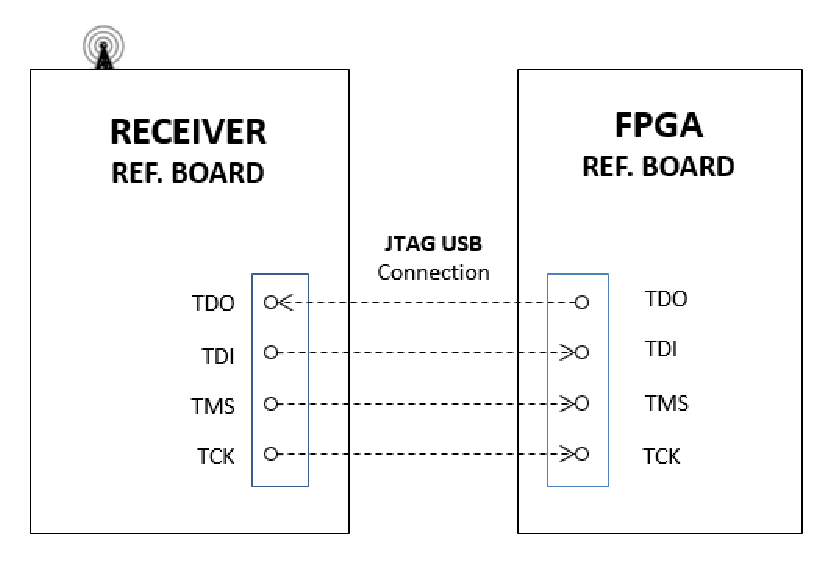
\includegraphics[width=2.7in]{images/Fig4.eps}
\caption{DTV Receiver (host) connected to a reference FPGA board (target), through a USB/JTAG programmer cable.}
\label{figure:fig4}
\end{figure}
%

%==============================================================
\section{The Hardware Reconfiguration Scheme Based on the DTV Signal}
\label{hardware-reconfig}
%==============================================================

The entire hardware reconfiguration scheme can be split into three distinct steps. The first step consists of preparing data to be broadcast. In particular, that means encapsulating the synthesized FPGA bit-stream into a transport stream. Here, it is assumed that the bit-stream is already synthesized, tested, and validated for the same FPGA model used by the receiver. The second step involves filtering, remounting, checksum validation, and persistence. The last step uses the downloaded bit-stream to reconfigure the receiver FPGA module. 
%All mentioned steps, which result in the complete reconfiguration process of the FPGA device, compose HARD. 
The following sections discuss each procedure step in detail.

%==============================================================
\subsection{Encapsulating Hardware Data}
\label{encap-method}
%==============================================================

In order to choose a transmission method for hardware reconfiguration modules, one must take into account data format and timing requirements. Regarding data format, as already mentioned, the possible classifications are: delimited, un-delimited, and datagrams. When addressing timing requirements, data can be synchronous, synchronized, and asynchronous. Table \ref{table:table-one} shows a summary of what was tackled in this work, regarding the data broadcasting mechanisms presented section \ref{data-broadcasting}.


%Need add the table -------- rribeiro
\begin{table}[ht]
\renewcommand{\arraystretch}{1.18}
\footnotesize{ !!!!!!!!ADD THIS TABLE!!!!!!!! }
\caption{Comparison Regarding Data Broadcasting Methods}
\label{table:table-one}
\end{table}

Ultimately, hardware cores are binary data, which contain hardware descriptions for configuring FPGA devices. As a result, the hardware reconfiguration stream is regarded as delimited data and can be split into slices of predetermined size. Moreover, it does not have temporal requirements and can be considered as asynchronous data.
%

Indeed, a great concern lies on the data recovery procedure, which must be reliable and provide error-detecting capability \cite{ref23}. Using carousels \cite{ref20,ref21}, there is infrastructure regarding data recovery; however, they use complex structures, which incur large overhead and high computational effort. MPE cannot be considered, due to its dependence on a network protocol, and data piping does not provide synchronization capability. Besides, hardware reconfiguration files are not complex, which suggests simple transport mechanisms. As a consequence, a good option is the data streaming through private sections approach, which is simple and already provides error-detection tools; and support to delimited and asynchronous data, with structures less complex than the ones used in carousels. In summary, the reconfiguration file can be partitioned in sections, which are enumerated according to their insertion order and cyclically repeated, as shown in Fig. \ref{figure:figcyc}.

\begin{figure}[ht]
\centering
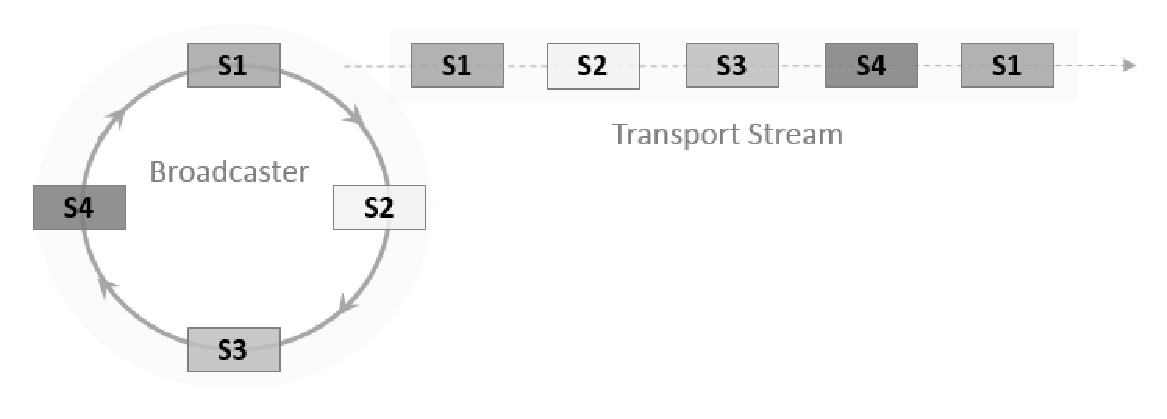
\includegraphics[width=3.4in]{images/cyc.eps}
\caption{Transmission strategy with private sections.}
\label{figure:figcyc}
\end{figure}


\subsection{Hardware Data Multiplexing in Transport Streams}\label{data-multiplexing}
From the point of view of the DTV signal, the FPGA bit-stream is seen as regular data. Thus, such content needs to be signaled ({\em i.e.}, a PID to identify the stream and a new data table), in order to notify the receiver about its existence, in the broadcast signal, following the DTV standard rules. First, it is necessary to choose a suitable method for transporting reconfiguration bit-streams, by taking into account their main characteristics, which was already done above and resulted in data streaming through private sections (see section \ref{encap-method}).



%Beyond what was tackled, other criteria for choosing the most suitable data broadcast method were taken into consideration: support for error detection and capability to perform broadcast. TABLE~\ref{table:table-one} compares the data piping, data streaming and carousel techniques, in order to check the most suitable method for this task. MPE was not considered here, due to its dependence on a network protocol (see section \ref{data-broadcasting}). Considering what is shown in TABLE~\ref{table:table-one}, the most appropriate data broadcasting method, for transporting hardware reconfiguration data, is data streaming using private sections.


Thus, the hardware bit-stream is divided into sections of $4092$ bytes in length, as illustrated in Fig.~\ref{figure:fig5}, according to the data streaming rules. The identification of the private section content is given by $table\_id$, which is an $8$-bit field of the private section table. The $section\_number$ field presents the sequential number of a section, which is used to keep the correct order for data remounting. It is worth noticing that sections can arrive out of order and, therefore, the resident receiver system needs to implement a mechanism to maintain the correct section order.

%
\begin{figure}[ht]
\centering
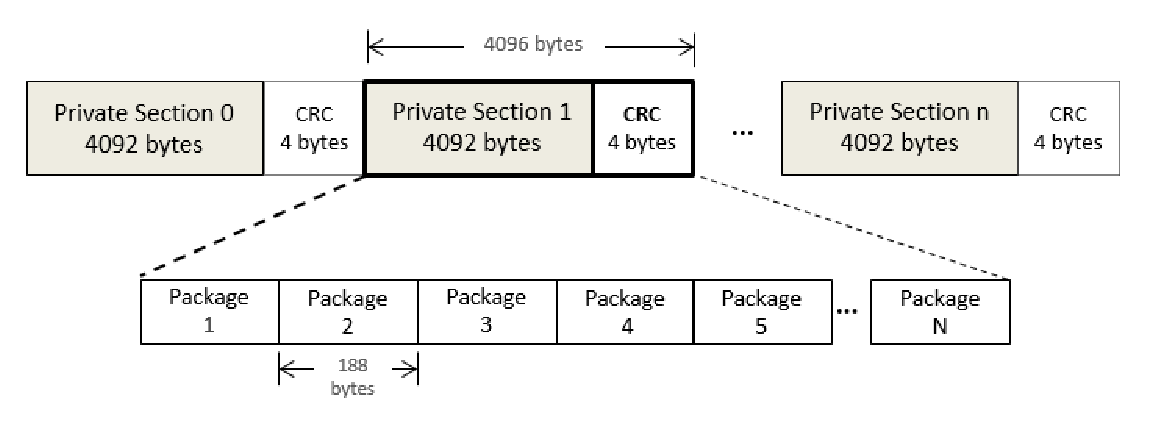
\includegraphics[width=3.4in]{images/Fig5.eps}
\caption{The FPGA synthesis stream, divided into sequenced private sections of variable size, which are then organized into TS packets.}
\label{figure:fig5}
\end{figure}
%


The $last\_section\_number$ field indicates the total number of sections used for carrying the synthesized hardware content. The $private\_data\_byte$ field is a variable-size one, which is used to carry the FPGA bit-stream. 

For this work, the $section\_syntax\_indicator$ field was set to `1', in order to enable the CRC\_32 checksum field of the private section syntax. This redundant information enables the receiver to detect errors, via a checksum algorithm.

In order to signal the FPGA bit-stream content, HARD follows a syntax similar to the one used by AIT. In summary, it must provide a FPGA bit-stream description and an access point, in such a way that the receiver is able to download and remount FPGA core data. The new table, named update information table (UIT), follows the AIT syntax. Its role is to provide detailed information about characteristics of the transmitted FPGA core. This is crucial information used by the receiver, in order to decide if the transmitted content can be used or not. The FPGA core information, borne by the new table, is then used by the receiving device, in order to filter the hardware bit-stream.

Other information, about the transmitted hardware core, must also be included and broadcast, along with hardware contents, such as a description of the hardware upgrade module ({\em e.g.}, decoder, multiplexer, and cypher.), FPGA manufacturer name, family, device part number (which was used to synthesize the core), size of the synthesized core, in bytes, PID and TID for section filtering. The mentioned data need to be added to the TS, in order to provide all necessary information related to the new content. TABLE~\ref{table:table-two} shows the complete UIT structure, whose mnemonics are define in the MPEG-2 systems standard~\cite{ref17}.

\begin{table}[ht]
\renewcommand{\arraystretch}{1}
\footnotesize{ !!!!!!!!ADD THIS TABLE!!!!!!!! }
\caption{The Update Information Table - UIT}
\label{table:table-two}
\end{table}

Program map table (PMT) sections provide the access point to the newly created UIT table, in a similar way as already done for AIT. UIT gives access to the $hw\_core\_flag$ field, which is used to signal the existence of hardware content. If this field is set to `0x1', this means that there is hardware content in the DTV signal; otherwise, `0x0' indicates that no hardware content is being broadcast.

The $fpga\_core\_number$ field identifies the number of hardware cores being currently broadcast. The other necessary data are provided by $update\_hw\_identifier()$, which is a specific descriptor regarding transmitted hardware modules, similar to $application\_identifier()$, used in AIT. The $update\_hw\_identifier()$ portion presents a list of available hardware cores, whose size was reported by $fpga\_core\_number$. The syntax of $update\_hw\_identifier()$ is shown in TABLE~\ref{table:table-three}.


\begin{table}[ht]
\renewcommand{\arraystretch}{1}
\footnotesize{ !!!!!!!!ADD THIS TABLE!!!!!!!! }
\caption{The update\_hw\_identifier Field Syntax}
\label{table:table-three}
\end{table}


The $fpga\_core\_size$ field is $32$ bits in length, informs the core size, and is used by the receiver application, in order to check if the whole bit-stream content was reassembled. The $fpga\_core\_version$ field identifies the core update version number and is used during the reassembling process, in order to check if the receiver was already updated. The following three fields are descriptors, which bear information about each transmitted core. In addition, there is a list of access points (PID and TID), which are used for filtering private sections carrying hardware-reconfiguration content (see TABLE~\ref{table:table-four}). 

TABLE~\ref{table:table-four} presents the syntax of the $fpga\_core\_module\_name()$ descriptor, which is identified by a $descriptor\_tag$ set to `0x01'.


\begin{table}[ht]
\renewcommand{\arraystretch}{1}
\footnotesize{ !!!!!!!!ADD THIS TABLE!!!!!!!! }
\caption{The FPGA\_core\_module\_name Descriptor Syntax}
\label{table:table-four}
\end{table}


The $descriptor\_length$ field identifies the size of the content located inside the loop. The next field, that is, $descriptor\_core\_length$, identifies the size of the $core\_module\_name$ information, where each character is coded with 8 bits. Such a field is used to inform the hardware module name ({\it e.g.}, decoders, multiplexer, and cypher) available for reconfiguration. The next descriptor is named $fpga\_core\_device\_info()$  and is shown in TABLE~\ref{table:table-five}. This descriptor is identified by a $descriptor\_tag$ set to `0x03'. Its $descriptor\_length$ field presents the size of the $fpga\_info$ string field, where each character is also coded with 8 bits. This field informs the name of the FPGA manufacturer, followed by the FPGA family and, lastly, the part number of the FPGA device, for which the core was synthesized. Such values are arranged into the $fpga\_info$ character string field, separated by spaces (`0x32'): ``fpga-manufacturer-name fpga-family-name fpga-part-number''. This information is used, by the receiver, to identify the FPGA device information in the broadcast content.

\begin{table}[ht]
\renewcommand{\arraystretch}{1}
\footnotesize{ !!!!!!!!ADD THIS TABLE!!!!!!!! }
\caption{The FPGA\_core\_device\_info Descriptor Syntax}
\label{table:table-five}
\end{table}

The last descriptor is $fpga\_section\_identifier()$, shown in TABLE~\ref{table:table-six}. This descriptor is identified by a $descriptor\_tag$ set to `0x05'. The next field, that is, $descriptor\_length$, contains the loop content size, in bytes. The $remount\_core\_pck\_pid$ field informs the PID used to locate packets with the desired hardware content. Besides, it is used, in association with the $remount\_core\_sec\_tid$ field (which informs the section table ID (TID)), for accessing private sections with core content. The $remount\_priority$ field informs the remount priority order for each group of $256$ sections, represented by its own PID and TID. Such an approach is used if the hardware bit-stream needs more than $256$*$4080$ bytes; otherwise, only one group is enough, that is, it is set to `0x00'. For the next group represented by other PIDs and TIDs, this value is incremented by $1$ and so on. 

The receiver system uses the presented information to check the characteristics of the broadcast hardware core and, if a match is found, also to guide the execution of hardware updates.

\begin{table}[ht]
\renewcommand{\arraystretch}{1}
\footnotesize{ !!!!!!!!ADD THIS TABLE!!!!!!!! }
\caption{The FPGA\_section\_identifier Descriptor Syntax}
\label{table:table-six}
\end{table}


%==============================================================
\subsection{Core Data Filtering}
\label{core-data}
%==============================================================

The DTV-receiver resident system is configured to filter the transmitted content, in order to find some hardware reconfiguration bit-stream (core). The system will look for UIT and parse it, beginning with the $hw\_core\_flag$ field. If it is set to `0x0', the system simply ignores the current UIT; otherwise (`0x1'), there is a signaled hardware bit-stream content and the system then parses the remaining UIT content ({\em e.g.}, $fpga\_core\_size$, $fpga\_core\_version$, and $fpga\_core\_module\_name()$), in order to retrieve the corresponding table fields, which describe the characteristics of the broadcast bit-stream (hardware core). Finally, such values are compared with those of the local FPGA devices, as shown in Fig.~\ref{figure:fig6}. The characteristics of the local FPGA devices can be stored in a simple text file, which is made available at the receiver file system, as done here.

%
\begin{figure}[ht]
\centering
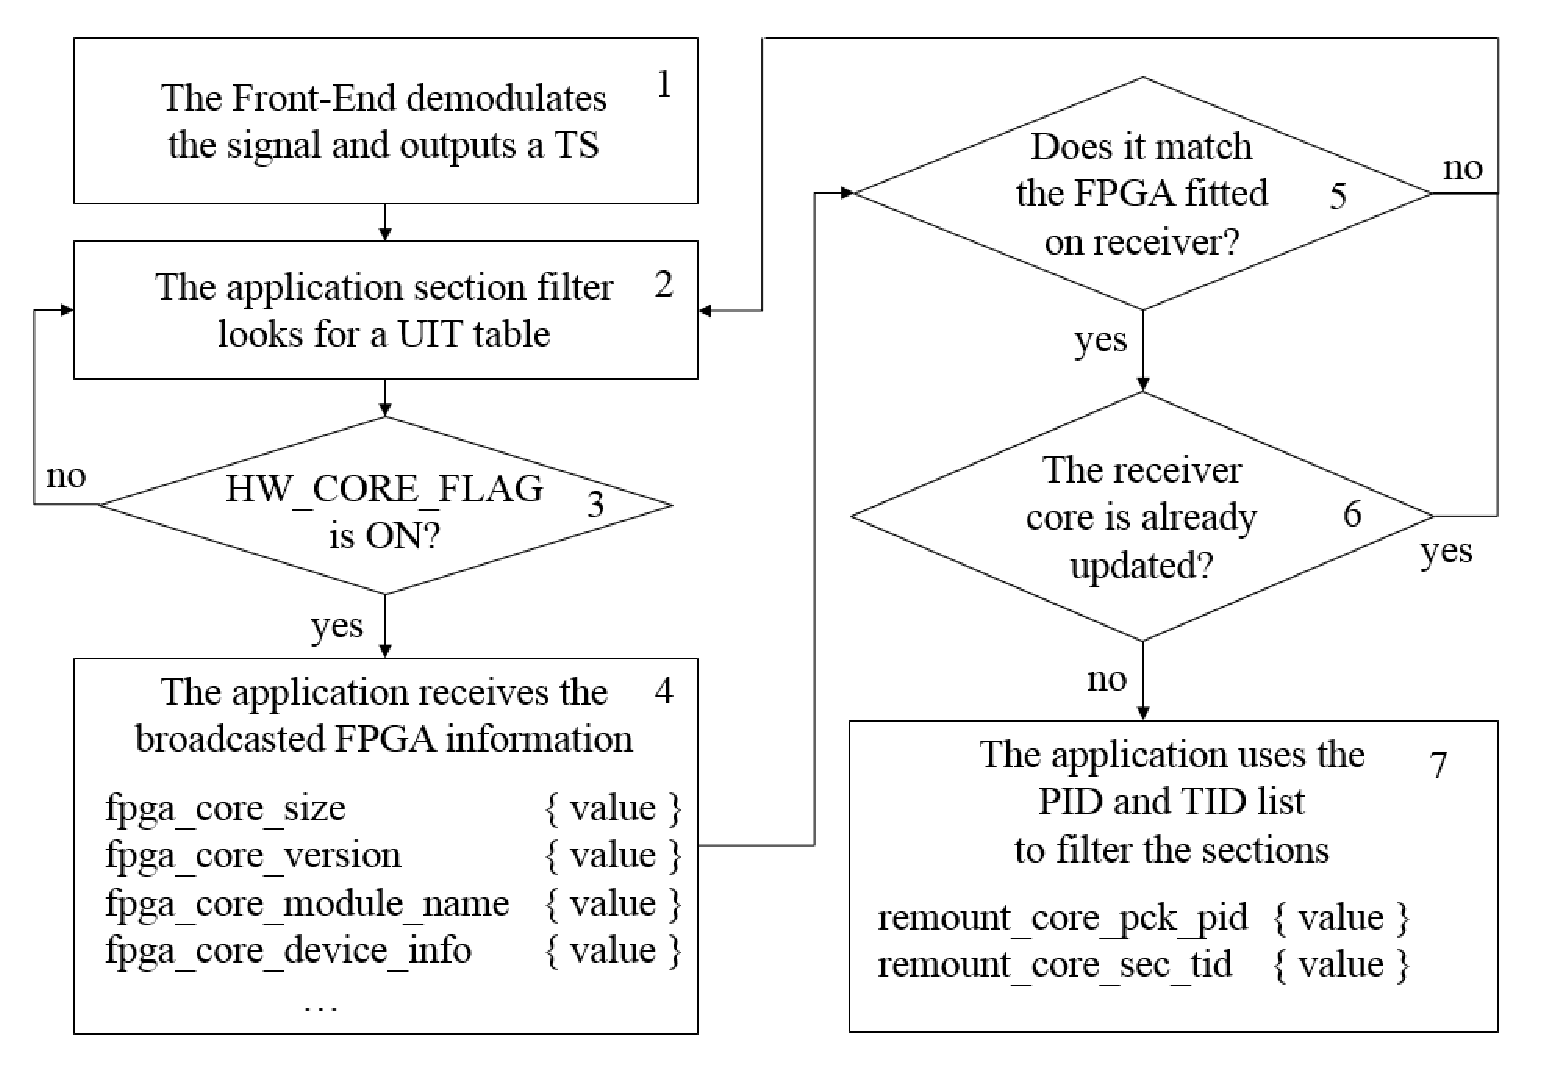
\includegraphics[width=3.4in]{images/Fig6.eps}
\caption{Steps to check the UIT content and find a broadcast core hardware suitable for the receiver, in order to retrieve the correct PID for filtering.}
\label{figure:fig6}
\end{figure}
%

One one hand, if some of these fields do not match the receiver hardware characteristics, the system then interrupts the reconfiguration process. Indeed, it may happen, given that content may have been sent to another kind of receiver, with different FPGA devices. On the other hand, if such content fits the receiver hardware architecture, then the system continues the filtering procedure and parses the $remount\_core\_pck\_pid$ and $remount\_core\_sec\_tid$ fields. Those values are used as an access point for extracting the transmitted reconfiguration bit-stream (for programming section-filter modules), directly from private sections, as depicted in Fig.~\ref{figure:fig7}. When a private section is retrieved, its CRC is checked, for validation purposes (see section \ref{data-broadcasting}). If the section is not corrupted, the system stores the section payload, according to the section order provided by the $section\_number$ field; otherwise, the system will wait for a new section.

The system keeps this iterative process until the last section is received, in order to conclude the reassembling process. However, the procedure completion depends on the validation of the entire private section payload. If a section is not validated ({\em e.g.}, corrupted), the reconfiguration process discards that and the search for a valid section content continues. Given that sections may be randomly retrieved, the receiving system is responsible for ensuring correct order.

%
\begin{figure}[hbt]
\centering
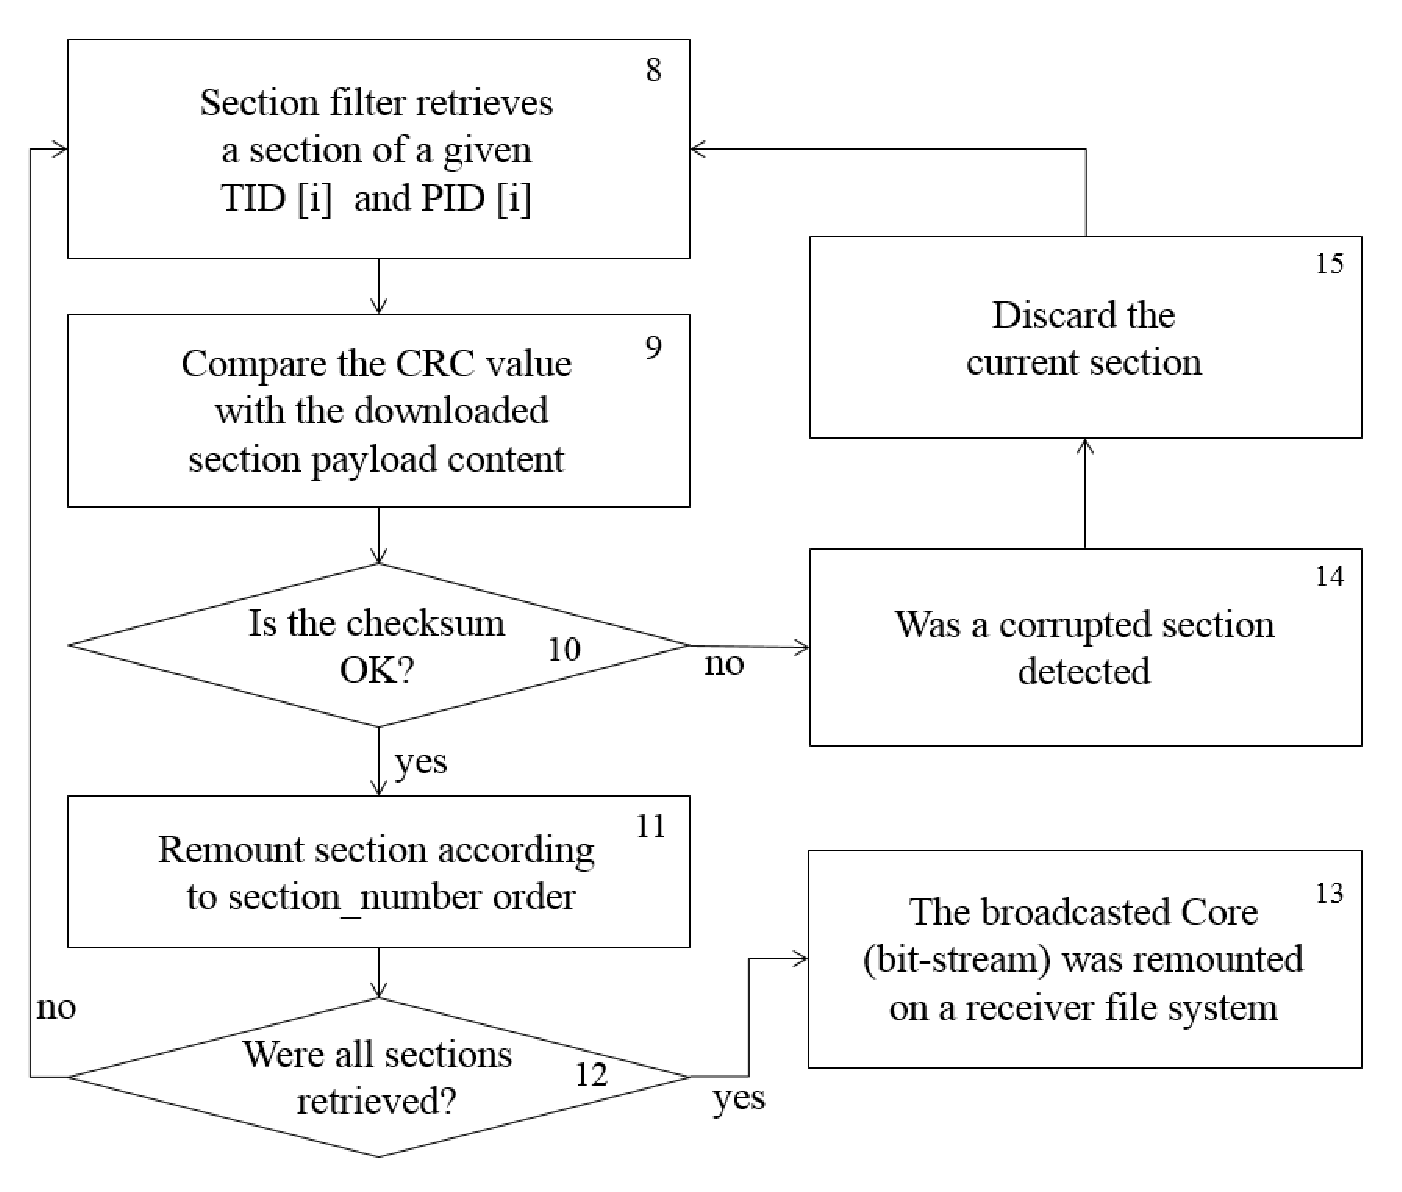
\includegraphics[width=3.4in]{images/Fig7.eps}
\caption{Steps involved in the process of obtaining the broadcast hardware core stream, which includes verification of each private section, downloading and content reassembling.}
\label{figure:fig7}
\end{figure}
%

%==============================================================
\subsection{The Target Device Reconfiguration}
\label{target-device}
%==============================================================

The FPGA reconfiguration is the last step of HARD. The main idea is to exercise the complete chain, that is, from the beginning of the process (core multiplexing) to its end (FPGA reconfiguration). At this point, the receiver has already checked if the core characteristics fit the FPGA model (see section \ref{core-data}), used at the receiver, and has finished the system core reassembling (obtained broadcast SVF file). Now, in this step, the remounted hardware core stream reaches a receiver reconfigurable target device, through a JTAG mode, as presented in section \ref{fpga-standalone} . 


%==============================================================
\subsection{Discussion about HARD}
\label{system-compatibility}
%==============================================================

Fig. \ref{figure:bigpicture} summarizes HARD, as explained in sections \ref{encap-method} to \ref{target-device}. As can be seen, it provides the transmission of pre-synthesized hardware cores, through MPEG-2 transport streams, in such a way that FPGA devices, integrated into commercial receivers, are addressed. Besides, the same content-transmission strategy already used for general data and SI ({\it e.g.}, tables and sections), in digital television systems \cite{dvbsi,isdbtsi}, is employed.


%
\begin{figure*}[htb]
\centering
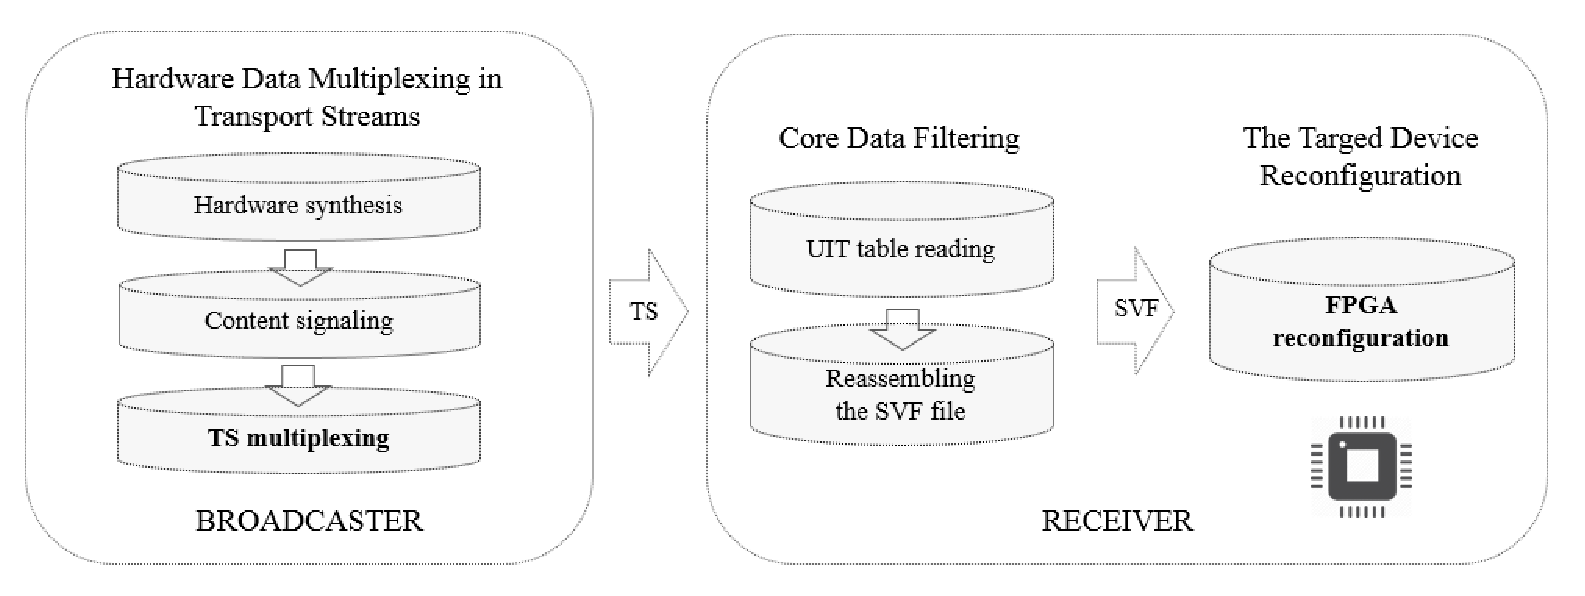
\includegraphics[width=5.1in]{images/bigpicture.eps}
\caption{All steps performed in HARD.}
\label{figure:bigpicture}
\end{figure*}
%

As one may notice, the presented reconfiguration system, at the receiver, is based on JTAG communication, SVF files, which are retrieved from the digital TV signal, and a newly created SI table (UIT) and its associated descriptors (see section \ref{data-multiplexing}), which are in charge of providing information regarding the hardware reconfiguration content. The SVF format is a standard used by almost all FPGA manufacturers and is compliant with the JTAG communication protocol. Additionally, the HARD SI-extension carries all necessary information regarding the FPGA device ({\it e.g.}, manufacturer, part number, and family identification) under update, which allows the complete identification of a given unit. As a consequence, it is not restricted to a specific manufacturer or FPGA model and is flexible enough in order to be adapted to other scenarios. For instance, nearly any given format could be sent in private sections as long as the related content is seen as a regular data flow.

Regarding content reception, the pre-synthesized core will be accepted only if there is a match between the information transmitted, which was filtered from UIT, and the locally available FPGA device; otherwise, the receiving system simply ignores the acquired content and waits for suitable data.

It is worth noticing that HARD presents some overhead, which is related to the encapsulation in private sections, that is, the private section header, and the SVF file format, which includes JTAG commands. The total overhead, is given by: $overhead = \left(N \times 16 \: \: bytes + 3 \: \: kbytes\right)$, where $N$ is the total number of sections necessary to carry the hardware content, $16$ bytes are the size of the private section header $\left(4096-4080 = 16\right)$, and $3$ kbytes is the size of SVF syntax and header file. 


HARD is based on an extension of SI standards \cite{dvbsi,isdbtsi}, without any modification regarding current structures, since it uses a new table (UIT) and associated descriptors, which were inspired by the AIT structure. Although that may sound intricate, its implementation is transparent and can even be done without a formal modification of the related standards, as a proprietary framework. Apart from that, the present approach addresses the complete update chain and provides a comprehensive and complete solution, which is still more feasible and simpler than isolated proprietary solutions or on-site maintenance.

Another interesting research topic about this work is security. Although it is not the focus of the present work, given that the main goals were to prove feasibility and also provide a complete and consistent framework, which could be readily used and further extended, some ideas may be tackled. Currently, there is a trend towards the adoption of security-by-design approaches, where built-in security tools are already available within the framework, that is, the system is designed from the ground up to be secure \cite{win8}. Another initiative is proof-carrying hardware (PCH), which may mitigate malicious code addition to IP modules, through the provision of functional specifications and security properties \cite{pch,pchmicro}. Actually, modules are validated by an automatic proof checker, through device code and the property proof. In summary, regarding HARD, security tools can be later added to the host system and other parts of the framework ({\it e.g.}, SI), in order to prevent hardware trojans or attacks to embedded systems.

Finally, the present proposal deals with evolution and standard update, which is directly related to resource availability for future hardware modules. Complexity measurements depend on many issues, like chosen platform and desired performance. Besides, the tool-set choices a standard is not necessarily coupled to the implementation complexity. For instance, regarding video coding, Bossen {\em et al} \cite{ref3} initially suggested that the software implementation cost of an HEVC decoder would not be much higher than that of an H.264/AVC one, although it is not obvious. In addition, one may notice that the number of used logic gates may be highly influenced by the parallelism supported by the HEVC standard \cite{hevc}. Consequently, given that IP developers already have a wide experience with previous solutions ({\it e.g.}, MPEG-1, MPEG-2, MPEG-4 AVC/H.264, and HEVC), they may be able to roughly predict future needs and then advise STB manufacturers, in order to integrate FPGA devices that may be updated for one or two future generations, for instance.


\subsection{Reconfiguration-Process Test Results}\label{reconfig-process}

As Proof of Concept (PoC), some HDL source code examples were synthesized, whose goal is to use the entire scheme. Four VHDL/Verilog source code examples are used, which were synthesized for a reference FPGA and then tested and validated, by means of an EDA tool.

The experimental setup, used in this work, includes a tool set necessary to validate all steps performed by HARD. In order to synthesize digital circuits, the tool Quartus II v.11.0, provided by the Altera FPGA manufacturer, was used. Such a tool is able to generate the reprogramming file in several formats, including the chosen one, that is, SVF. The advanced stream combiner (ASC) tool, provided by the manufacturer Rohde \& Schwarz, was employed to multiplex content in a transport stream. During the creation of the transport stream, UIT was added and the SVF content was split and encapsulated into private sections. Modulation and broadcast were achieved by using a VHF/UHF modulator (DekTec DTU-215, USB-2 device), with a companion player tool (StreamXpress v.3.10.2, also provided by DekTec). The receiver device used for test and development was a NXP-STB225 IP and hybrid DTV STB platform, which was provide by NXP semiconductors. The mentioned platform runs a version of the Linux operating system, on a dual core $300$ MHz MIPS processor. Finally, the employed FPGA device was a Nios Stratix EP1S10F780C6 development board, which was developed by Altera and runs at $50$ MHz.

The validation is based on typical examples, in order to check if the FPGA is configured properly and the scheme works in a DTV system. The first pre-synthesized example converted to an SVF file (see section \ref{hardware-data}) is a simple binary-coded decimal (BCD) light emitting diode (LED) counter (Ex01.svf). The second one is a BCD to $7$-Seg decoder (Ex02.svf). The third is an example that writes a text message on a 16x2 liquid crystal display (LCD) device (Ex03.svf). Finally, the fourth and last one is a $7$ segments counter (Ex04.svf).

Each core is multiplexed into its respective TS, according to the schema described in this work (see sections \ref{encap-method} to \ref{target-device}). The result of this process consists of fourth transport stream files, carrying and signaling each respective bit-stream. The mentioned TS example files are generated according to the integrated services digital broadcasting terrestrial (ISDB-T) standard~\cite{ref33}, which is similar to terrestrial DVB. For this process, the mentioned MPEG2 transport stream data generator and packet manipulator tool was employed. The bit rate used to multiplex each transport stream is $1.57$ Mbps.

The first set of experiments was performed to establish the best section repetition rate to be used in HARD. Regarding that, $8$ transport streams, carrying and signaling Ex01.svf hardware core, were generated. Thus, for the first example, the repetition rate used was $500$ms. Next, $750$ms, $1000$ms, $1250$ms, $1500$ms, $1750$ms, and $2000$ms repetition rates were successively tested (see TABLE~\ref{table:table-seven}).


\begin{table}[ht]
\renewcommand{\arraystretch}{1}
\footnotesize{ !!!!!!!!ADD THIS TABLE!!!!!!!! }
\caption{Remounting time values obtained for the first pre-synthesized example, using different repetition rates.}
\label{table:table-seven}
\end{table}


According to TABLE~\ref{table:table-seven}, the results using a rate of $500$ms (Ex01\_$500$ms.ts) presented the lowest performance, during the remounting process with private sections. Using this specific rate, there is a greater discard of sections by the remounting system, when compared with lower rates. Such a discard happens when the remounting system captures a smaller number of sections, in each repetition cycle. Using the $750$ms repetition rate (Ex01\_$750$ms.ts), there was an improvement in the remounting performance, due to the reduced discard of sections, when compared with the $500$ms repetition rate. However, rates between $1000$ms and $1500$ms presented the best average performance during the hardware core remounting procedure. It is worth noticing that the mentioned rates provided similar remounting times, but with a clear trend towards an increase in this merit figure.

The other experiments were based on a private section bit-rate of $1000$ms; the UIT bit-rate is also $1000$ms. In order to perform the TS broadcasting task, the mentioned USB $2.0$-based multi-standard modulator was used.

Some results were generated for validating the correct operation of the entire scheme. The metrics evaluated here, whose goal is to give an idea about the obtained performance, are the remounting time (RMT), that is, the time during the download of the reconfiguration data, and the reconfiguration time (RCT), which is the time period employed to parse the related SVF file and reconfigure the target FPGA. The latter will take place only if a RMT process has occurred. The RMT is the sum of the checksum verification time, necessary to check all sections, and the download time for all sections (remounting). The RCT time is the total time needed to reconfigure the FPGA device, using the implemented JTAG host/target mode. TABLE~\ref{table:table-eight} shows the obtained results, when broadcast and reception tests were performed, using this reconfiguration scheme. The pre-synthesized core file name is represented by the HWNAME table column. Column CRSIZE shows the pre-synthesized core size, followed by the TSNAME, which is the generated transport stream file name. Finally, the RMT and RCT fields show the obtained average remounting time and average reconfiguration time values, respectively.

\begin{table}[ht]
\renewcommand{\arraystretch}{1.18}
\footnotesize{ !!!!!!!!ADD THIS TABLE!!!!!!!! }
\caption{Remounting and reconfiguration time values obtained for all the employed pre-synthesized examples, using a $1000$ms repetition rate}
\label{table:table-eight}
\end{table}

The performed experiments showed that pre-synthesized cores could be signaled, multiplexed, and broadcast with other DTV contents. The achieved RMT time, in each experiment, is satisfactory, considering that the scheme's task was performed in concurrency with other DTV tasks ({\em e.g.}, application retrieval, table filtering, and electronic program guide construction). The RCT is also satisfactory, considering that the employed reference receiver presents low processing power. Indeed, the SVF parser took most of the elapsed time. The reconfiguration JTAG mode is generic and ideal for this PoC, but can be improved if FPGA devices are integrated into the receiver board.

The RMT associated to Ex02.svf was larger than what was obtained with the other example files, due to the way this particular reconfiguration bit-stream is organized into sections. Although all test files present the same size, the resulting RMT depends on some factors, such as start point related to private sections, signal strength, and corrupted private sections. Regarding final users, those periods are not perceived, given that associated tasks are performed in parallel with other receiver tasks. However, if the reconfigured FPGA device is being used ({\em e.g.}, for media decoding), a momentary service interruption may be noticed.

The reconfiguration scheme through the DTV signal, presented here, can be regarded as an innovative approach, when compared to those found in the literature on reconfigurable architectures. The main idea of HARD relies on the delivering methodology for pre-synthesized hardware cores. 

Recent studies (see section related-work) use pre-synthesized cores, for run-time reconfiguration, and present some similarities with HARD. The main difference is that the former needs to maintain a number of previously stored cores; then, the resident system decides when to use each one. HARD, however, can broadcast the desired core to a huge number of devices, which are then automatically reconfigured. In addition, this scheme could send pre-synthesized cores of several manufacturers, and each device would then be responsible for accepting or rejecting such content.

Another feature is that a broadcaster can send the hardware update data cyclically, during a period of time, which provides an opportunity for all devices, in the range of the DTV signal, to perform hardware reconfiguration. Thus, in DTV networks, where receivers are based on the replacement of hardware modules, the new technology advances and enhancements could be immediately incorporated, leading to a flexible DTV environment.

%================================
\section{Conclusions}
\label{conclu}
%================================

This work presents a new approach for hardware reconfiguration, which is intended to be used in DTV environments. HARD allows the receiver to be automatically reconfigured, providing an approach to create new receiver architectures. Additionally, the receiver design architecture could be focused on hardware upgrade, in numerous ways.

The results obtained with the pre-synthesized core experiments show that the system is able to reconfigure distinct core modules, in a DTV system. The experiments also show that this reconfiguration scheme can work in parallel with other DTV tasks. Indeed, the obtained remounting time is satisfactory, considering embedded systems with low processing power, and the reconfiguration time can be improved, if the FPGA is integrated into the receiver board. 

Tests using media decoders were not performed, but there is no restriction regarding that, since HARD is able to update any hardware module, as long as the structure described in section \ref{hardware-reconfig} is followed. Additionally, the chosen examples are simple enough, in order allow fast implementation and easy multiplexing, and complex enough, in such a way that the complete hardware update chain is used, with the goal to reveal its complexity and also to show its validity.

Critical tasks normally performed by an ASIC device, such as H.$264$ video decoding and cryptography tasks, could be designed for FPGA devices, based on the present scheme. It would enable the incorporation of technological advances, such as new video compression schemes, which would create a flexible DTV network. Furthermore, other devices that use transport streams could also make use of HARD, in order to design intelligent architectures and flexible low-cost devices.

It is worth noticing that the overhead presented by the proposed methodology is largely affected by the pre-synthesized file format. Universal formats, such as SVF, include more information in the file header, which increases the final file size. Consequently, many private sections would be needed and the remounting process, at the receiver, would be slower. Indeed, regarding the latter, it is necessary to parse the reconfiguration file, in order to extract the SVF syntax. It is done before the reconfiguration process itself, which increases the system overhead. The associated file overhead may be reduced by using proprietary/dedicated reconfiguration schemes, however, the universal behavior of such a scheme is lost.


%\begin{acknowledgements}
%If you'd like to thank anyone, place your comments here
%and remove the percent signs.
%\end{acknowledgements}

% BibTeX users please use one of
%\bibliographystyle{spbasic}      % basic style, author-year citations
%\bibliographystyle{spmpsci}      % mathematics and physical sciences
%\bibliographystyle{spphys}       % APS-like style for physics
%\bibliography{}   % name your BibTeX data base

% Non-BibTeX users please use
\begin{thebibliography}{}
%
% and use \bibitem to create references. Consult the Instructions
% for authors for reference list style.
%

\bibitem{ref1}
D. Yoshida, M. Takahashi, H. Mizosoe, T. Nakamura, and Y. Yatabe,``Highly efficient H.264/AVC codec technology for high definition consumer applications,'' in \emph{Proc. IEEE International Conference on Consumer Electronics}, Las Vegas, Nevada, USA, pp. 1-2, Jan. 2008.

\bibitem{ref2}
G. J. Sullivan, J. R. Ohm, W.-J. Han, and T. Wiegand, ``Overview of the high efficiency video coding (HEVC) standard,'' \emph{IEEE Transactions on Circuits and Systems for Video Technology}, vol. 22, no. 12, pp. 1649-1668, Sep. 2012.
	
\bibitem{ref3}
F. Bossen, B. Bross, K. Sühring, and D. Flynn, ``HEVC complexity and implementation analysis,'' \emph{IEEE Transactions on Circuits and Systems for Video Technology}, vol. 22, no. 12, pp. 1685-1696, Oct. 2012.
	
\bibitem{ref4}
	H. Koumaras, M. Kourtis, and D. Martakus, ``Benchmarking the encoding efficiency of H.265/HEVC and H.264/AVC,'' in \emph{Proc. Future Network \& Mobile Summit}, Berlin, Germany, pp. 1-7, Jul. 2012.
	
\bibitem{ref5}
IEEE Standard, ``IEEE standard VHDL language reference manual,'' IEEE Std 1076-2008, Jan. 2009.
	
\bibitem{ref6}
IEEE Standard, ``IEEE standard for verilog hardware description language,'' IEEE Std 1364-2005, Apr. 2006.

\bibitem{ref7}
S. Z. Ahmed, G. Sassatelli, L. Torres, and L. Roug\'e, ``Survey of new trends in industry for programmable hardware: FPGAs, MPPAs, MPSoCs, structured ASICs, eFPGAs and new wave of innovation in FPGAs,'' in \emph{Proc. International Conference on Field Programmable Logic and Applications}, Milano, Italy, pp. 291-297, Sep. 2010.

\bibitem{ref8}
B. K. Reddy, S. Sabbavarapu, and A. Acharyya, ``A new VLSI IC design automation methodology with reduced NRE costs and time-to-market using the NPN class Representation and functional symmetry,'' in \emph{Proc. IEEE International Symposium on Circuits and Systems}, Melbourne, Australia, pp. 177-180, Jun. 2014.

\bibitem{ref9}
P. H. W. Leong, ``Recent trends in FPGA architectures and applications,'' in \emph{Proc. IEEE International Symposium on Electronic Design, Test and Applications}, Hong Kong, SAR, China, pp. 137-141, Jan. 2008. 

\bibitem{ref10}
E. Monmasson and M. N. Cirstea, ``FPGA design methodology for industrial control systems - A review,'' \emph{IEEE Transactions on Industrial Electronics}, vol. 54, no. 4, pp. 1824-1842, Aug. 2007.
	
\bibitem{ref11}
A. H. Salman, T.  Adiono,  W. A. Cahyadi,  Y. Kurniawan, ``SOC design and FPGA implementation of Digital TV receiver,'' in \emph{Proc. International Conference on Telecommunication Systems, Services, and Applications}, Bali, Indonesia, pp. 125-129, Oct. 2012.
	
\bibitem{ref12}
ABNT Standard, ``Digital terrestrial television, video coding, audio coding and multiplexing Part 3: Signal multiplexing systems,'' ABNT NBR 15602-3, Nov. 2007.
	
\bibitem{ref13}
C.-T. Lin, S.-J. Horng, and Y.-L. Huang, ``Hardware resource manager for reconfiguration system,'' in \emph{Proc. International Symposium on Biometrics and Security Technologies}, Taipei, Taiwan, pp. 59-65, Mar. 2012.
		
\bibitem{ref14}
J. Eachanobe, I. Del Campo, R. Finker, and k. Basterretxea, ``Dynamic Partial Reconfiguration in embedded systems for intelligent environments,'' in \emph{Proc. IEEE International Conference on Intelligent Environments}, Guanajuato, Mexico, pp. 26-29, Jun. 2012.
	
\bibitem{ref15}
D. Hillenbrand, C. Brugger, J. Tao, S. Yang, and M. Balzer, ``RIVER: reconfigurable pre-synthesized-streaming architecture for signal processing on FPGAs,'' in \emph{Proc. IEEE Parallel and Distributed Processing Symposium Workshops \& PhD Forum}, Shanghai, China, pp. 397-400, May 2012.

\bibitem{ref16}
O. Serres, V. K. Narayana, and T. El-Ghazawi, ``An architecture for reconfigurable multi-core explorations,'' in \emph{Proc. International Conference on Reconfigurable Computing and FPGAs}, Cancun, Mexico, pp. 105-110, Dec. 2011.

\bibitem{refX1}
Y. Wang, X. Zhou, L. Wang, J. Yan, W. Luk, C. Peng, and J. Tong ``SPREAD: A streaming-based partially reconfigurable architecture and programming model,'' in \emph{Proc. IEEE Transactions Very Large Scale Integration (VLSI) Systems}, vol. 21, no. 12, pp. 2179-2192, Jan. 2013.

\bibitem{ref34}
S. S. Bhattacharyya, J. Eker, J. W. Janneck, C. Lucarz, M. Mattavelli, and M. Raulet, ``Overview of the mpeg reconfigurable video coding framework,'' \emph{Journal of Signal Processing Systems}, vol. 63, no. 2, pp. 251-263, May 2011.

\bibitem{ref40}
M. Mattavelli,  I. Amer, and M. Raulet, ``The reconfigurable video coding standard,'' {\it IEEE Signal Processing Magazine}, vol. 27, no. 3, pp. 159-167, May 2010.

\bibitem{ref37}
J. Nezan, N. Siret, M. Wipliez, F. Palumbo, and L. Raffo,`` MultiPurpose
systems: a novel dataflow-based generation and mapping strategy,'' in {\it Proc. International Symposium on Circuits and Systems}, Seoul, Korea, pp. 3073-3076, May 2012.

\bibitem{ref35}
E. Bezati, S. Casale-Brunet, M. Mattavelli, and J. W. Janneck, ``Synthesis and optimization of highlevel stream programs,'' in {\it Proc. Electronic System Level Synthesis Conference}, Austin, USA, pp. 1-6, May 2013.

\bibitem{ref36}
J. W. Janneck, I. D. Miller, D. B. Parlour, G. Roquier, M. Wipliez, and M. Raulet, ``Synthesizing hardware from dataflow programs: an MPEG-4 simple profile decoder case study,'' {\it Journal of Signal Processing Systems}, vol. 63, no. 2, pp. 241-249, May 2011.

\bibitem{ref39}
G. Roquier, M. Wipliez, M. Raulet, J.-F. Nezan, and O. Deforges, ``Software synthesis of CAL actors for the MPEG reconfigurable Video Coding framework,'' in {\it Proc. IEEE International Conference on Image Processing}, San Diego, USA, pp. 1408-1411, Oct. 2008.

\bibitem{ref41}
M. Wipliez, G. Roquier, J.-F. Nezan, ``Software Code Generation for the RVC-CAL Language,'' {\it Journal of Signal Processing Systems}, vol. 63, no. 2, pp. 203-213, May 2011.

\bibitem{ref38}
C. Sau, L. Raffo, F. Palumbo, E. Bezati, S. Casale-Brunet, and M. Mattavelli, ``Automated design flow for coarsegrained reconfigurable platforms: an RVC-CAL multistandard decoder usecase,'' in {\it Proc. International Conference on Embedded Computer Systems: Architectures, Modeling, and Simulation}, Agios Konstantinos, Greece, pp. 59-66, July 2014.

\bibitem{ref17}
ISO/IEC International Standard, ``Information technology - Generic coding of moving pictures and associated audio information: systems,'' ISO/IEC 13818-1, Dec. 2000.

\bibitem{ref18}
ABNT Standard, ``Digital terrestrial television, data coding and transmission specification for digital broadcasting part 3: data transmission specification,'' ABNT NBR 15606-3, Mar. 2012.

\bibitem{ref19}
M. S. Park, Y. J. Lee, J. H. Choi, and J. S. Choi, ``The design and implementation of data server for data broadcast service,'' in \emph{Proc. International Conference on Electronics, Circuits and Systems}, Sharjah, United Arab Emirates, vol. 3, pp. 1176-1179, Dec. 2003.

\bibitem{ref20}
E. P. J. Tozer, {\it Broadcast Engineer's Reference Book}, Focal Press: Burlington, USA, 2004, pp. 352-355.
	
\bibitem{ref21}
W. Fischer, {\it Digital Video and Audio Broadcasting Technology: A Practical Engineering Guide}, Springer Verlag: Berlin, Germany, 2010, pp. 457-465.
	
\bibitem{ref22}
G. Castagnoly, S. Brauer and M. Herrmann, ``Optimization of cyclic redundancy-check codes with 24 and 32 parity bits,'' \emph{IEEE Transactions on Communications}, vol. 41, no. 6, pp.883-892, Jun. 1993.

\bibitem{ref23}
U. Reimers, {\it DVB - The Family of International Standards for Digital Video Broadcasting}, 2nd~ed., Springer Verlag: Berlin, Germany, 2005, pp. 287-288.
	
\bibitem{ref24}
Digital Video Broadcasting, ``Specification for data broadcasting,'' ETSI EN 301 192 - V1.5.1, Nov. 2009.

\bibitem{ref25}
Digital Video Broadcasting, ``Implementation guidelines for Data Broadcasting,'' ETSI TR 101 202 - V1.2.1, Jan. 2003.

\bibitem{ref26}
R. J. Crinon, ``The DSM-CC object carousel for broadcast data services,'' in \emph{Proc. IEEE International Conference on Consumer Electronics}, Rosemont, USA, pp. 246-247, Jun. 1997.

\bibitem{ref27}
ABNT Standard, ``Digital terrestrial television - receivers,'' ABNT NBR 15604, Nov. 2007.
	
\bibitem{ref28}
E. Stavinov, {\it 100 Power Tips For FPGA Designers}, CreateSpace Independent Publishing Platform: Charleston, USA, 2011, pp. 171-200.
	
\bibitem{ref29}
IEEE Standard, ``IEEE standard for test access port and boundary-scan architecture,'' IEEE Std. 1149.1, 2013.
	
\bibitem{ref30}
M. Strubel, ``Implementing JTAG debugging solutions for custom hardware,'' in \emph{Proc. Embedded World 2012}, Nuremberg, Germany, pp. 1-17, Feb. 2012.
		
\bibitem{ref31}
R. Dominic, ``Design and implementation of an on-chip debug solution for embedded target systems based on the ARM7 and ARM9 family,'' Ph.D. thesis, University of Applied Sciences Augsburg, Augsburg, Germany, 2005.
		
\bibitem{ref32}
K. P. Parker, {\it The Boundary-Scan Handbook}, 3rd~ed., Kluwer Academic Publishers: Massachusetts, USA, 2003, pp. 10-60.

\bibitem{ref33}
ARIB Standard, ``Transmission system for digital terrestrial television broadcasting,'' ARIB STD-B31, Nov. 2005.

\bibitem{dvbsi}
Digital Video Broadcasting, ``Specification for service information (SI) in DVB systems,'' ETSI EN 300 468  - V1.14.1, May. 2014.

\bibitem{isdbtsi}
ARIB Standard, ``Service Information for Digital Broadcasting System,'' ARIB STD-B10 -  V4.6-E2, Jun. 2008.

\bibitem{win8}
J. Souren, ``Security by design: hardware-based security in Windows 8,'' \emph{Computer Fraud \& Security}, vol. 2013, no. 5, pp. 18-20, May 2013.

\bibitem{pch}
E. Love, Y. Jin, and Y. Makris, ``Proof-carrying hardware intellectual property: A pathway to trusted module acquisition,'' \emph{IEEE Transactions on Information Forensics and Security}, vol. 7, no. 1, pp. 25-40, 2012.

\bibitem{pchmicro}
Y. Jin and Y. Makris, ``A proof-carrying based framework for trusted microprocessor IP,'' in \emph{Proc. IEEE/ACM International Conference on Computer-Aided Design}, San Jose, USA, pp. 824-829, Nov. 2013.

\bibitem{hevc}
ISO/IEC International Standard, ``Information technology -- high efficiency coding and media delivery in heterogeneous environments -- part 2: high efficiency video coding,'' ISO/IEC 23008-2, May. 2015.


%\bibitem{RefJ}
% Format for Journal Reference
%Author, Article title, Journal, Volume, page numbers (year)
% Format for books
%\bibitem{RefB}
%Author, Book title, page numbers. Publisher, place (year)
% etc


\end{thebibliography}

\end{document}
% end of file template.tex

